% AWS-Native MCP/RAG Platform: Porting AI-Assisted Development Infrastructure
% to Managed Cloud Services
% Technical Paper - April 2026
\documentclass[11pt,letterpaper]{article}

% Packages
\usepackage[utf8]{inputenc}
\usepackage[margin=1in]{geometry}
\usepackage{amsmath,amssymb}
\usepackage{algorithm}
\usepackage{algorithmic}
\usepackage{listings}
\usepackage{xcolor}
\usepackage{hyperref}
\usepackage{booktabs}
\usepackage{graphicx}
\usepackage{tikz}
\usepackage{pgfplots}
\usepackage{fancyhdr}
\usepackage{enumitem}
\usepackage{multirow}
\usepackage{tabularx}
\usepackage{forest}
\usepackage{subcaption}
\usepackage{longtable}
\usepackage{pdflscape}
\usepackage{float}

\pgfplotsset{compat=1.18}

\usetikzlibrary{shapes.geometric, arrows.meta, positioning, fit, backgrounds, calc,
                 decorations.markings, patterns, shadows, matrix, chains}

% Custom colors
\definecolor{awsorange}{HTML}{FF9900}
\definecolor{awsblue}{HTML}{232F3E}
\definecolor{awslightblue}{HTML}{1B9CE5}
\definecolor{vpcgreen}{HTML}{248814}
\definecolor{neptuneblue}{HTML}{2E73B8}
\definecolor{opensearchpurple}{HTML}{9B59B6}
\definecolor{ecsgreen}{HTML}{27AE60}
\definecolor{cognitored}{HTML}{E74C3C}
\definecolor{s3yellow}{HTML}{F1C40F}
\definecolor{cdkpink}{HTML}{E91E63}
\definecolor{noaablue}{HTML}{003087}
\definecolor{dockerblue}{HTML}{2496ED}
\definecolor{chromagreen}{HTML}{2ECC71}
\definecolor{neo4jgreen}{HTML}{018BFF}
\definecolor{kiropurple}{HTML}{7B2FBE}

% Hyperref setup
\hypersetup{
    colorlinks=true,
    linkcolor=noaablue,
    citecolor=noaablue,
    urlcolor=awslightblue,
    pdftitle={AWS-Native MCP/RAG Platform},
    pdfauthor={NOAA MDC Global Workflow MCP Team},
    pdfkeywords={MCP, AWS, Neptune, OpenSearch, RAG, GraphRAG, ECS Fargate, CDK,
                 Bedrock Embeddings, Spec-Driven Development, Kiro}
}

% Code listing setup
\lstset{
    basicstyle=\ttfamily\footnotesize,
    breaklines=true,
    frame=single,
    captionpos=b,
    numbers=left,
    numberstyle=\tiny\color{gray},
    keywordstyle=\color{blue},
    commentstyle=\color{green!60!black},
    stringstyle=\color{red},
    backgroundcolor=\color{gray!5},
    showstringspaces=false
}

% Header/Footer
\pagestyle{fancy}
\fancyhf{}
\rhead{AWS-Native MCP/RAG Platform}
\lhead{NOAA MDC Global Workflow Team}
\cfoot{\thepage}

% Title information
\title{\textbf{AWS-Native MCP/RAG Platform:} \\
       \textbf{Porting AI-Assisted Development Infrastructure} \\
       \textbf{to Managed Cloud Services} \\[0.5em]
       \large From Docker Compose to Neptune, OpenSearch, and ECS Fargate \\
       \large with Spec-Driven Development via Kiro}

\author{
    Terrence McGuinness \\
    Modeling Development Center \\
    National Weather Service, NOAA \\
    \texttt{Terry.McGuinness@noaa.gov}
}

\date{April 16, 2026}

\begin{document}

\maketitle

\begin{abstract}
We describe the design and implementation of a complete port of the MDC
MCP/RAG Server---a 51-tool AI development platform for NOAA's Global
Forecast System---from a Docker Compose stack on virtual machines to
AWS-native managed services. The port replaces ChromaDB with Amazon
OpenSearch Service (vector search with k-NN), Neo4j with Amazon Neptune
(graph queries via openCypher), and Docker containers with ECS Fargate
behind a Private API Gateway. The system operates entirely within a VPC
with no Internet Gateway, complying with NOAA security policy. An adapter
pattern in the data access layer enables transparent backend switching
(\texttt{DB\_BACKEND=aws|legacy}) with zero changes to the 51 MCP tool
implementations. We present the migration methodology---driven by Kiro's
Spec-Driven Development system across 7 formal specifications---the APOC
procedure transformation engine for Neptune compatibility, the
multi-model embedding pipeline supporting both local sentence-transformers
and AWS Bedrock Titan/Nova models, and the Graph-Guided Semantic Retrieval
(GGSR) algorithm operating on a 59,759-node knowledge graph with 2.6
million relationships. The platform serves as a reference architecture for
porting COTS AI tooling to secure, private AWS environments. We further
describe advanced capabilities on the horizon: Matryoshka adaptive-dimension
embeddings, self-improving retrieval via drift detection and domain-adaptive
fine-tuning, SageMaker compute offloading, and the Kiro Spec-Driven
Development methodology that governed the entire 52-phase evolution of
this system.

\textbf{Keywords:} Model Context Protocol, AWS, Neptune, OpenSearch,
GraphRAG, ECS Fargate, CDK, Private API Gateway, Bedrock Embeddings,
Spec-Driven Development, Kiro, Matryoshka Embeddings, GGSR
\end{abstract}

\tableofcontents
\newpage

%===============================================================================
\section{Introduction}
%===============================================================================

\subsection{Motivation}

The NOAA Global Forecast System (GFS) is among the world's most complex
operational weather prediction systems, comprising over 4 million lines of
Fortran, Python, Shell, and C++ code across 30+ repositories. AI-assisted
development of this codebase requires deep structural understanding---not
just text search, but graph-aware retrieval that can trace a J-Job script
through shell wrappers into Fortran subroutine call chains spanning UFS,
NCEPLIBS, JEDI, and CMEPS frameworks.

Since October 2025, the MDC MCP/RAG Server has provided this capability
through the Model Context Protocol (MCP), serving 51 tools across 9 modules
to AI assistants (VS Code Copilot, Claude Desktop, Kiro, LangFlow). The
original deployment ran on NOAA Parallel Works virtual machines using Docker
Compose to orchestrate ChromaDB (vector search), Neo4j (graph database),
and a Node.js MCP server behind the Docker MCP Gateway.

This paper describes the complete port of that infrastructure to AWS-native
managed services, motivated by three requirements:

\begin{enumerate}[noitemsep]
    \item \textbf{Security compliance}: NOAA's AWS environment requires
          VPC-only access with no Internet Gateway---the Docker MCP Gateway's
          HTTP endpoint on port 18888 via dev tunnels cannot meet this
          requirement in production.
    \item \textbf{Operational maturity}: Docker Compose on ephemeral VMs
          requires manual reprovisioning after every VM restart; managed
          services eliminate this operational burden.
    \item \textbf{Scalability}: The single-container architecture cannot
          scale beyond one concurrent session; ECS Fargate with auto-scaling
          supports 1--4 tasks based on request volume.
\end{enumerate}

\subsection{System Evolution: 52 Phases in 6 Months}

The platform has evolved through 52 development phases since October 2025,
tracked via the Spec-Driven Development (SDD) methodology. Table~\ref{tab:evolution}
summarizes the major milestones.

\begin{table}[H]
\centering
\footnotesize
\begin{tabular}{@{}clll@{}}
\toprule
\textbf{Phase} & \textbf{Date} & \textbf{Milestone} & \textbf{Tools} \\
\midrule
1--10  & Oct--Nov 2025 & Initial MCP server, ChromaDB, 21 tools & 21 \\
11     & Dec 2025      & Docker MCP Gateway integration & 32 \\
23     & Jan 2026      & Static mode multi-user gateway & 32 \\
24E    & Feb 2026      & Hierarchical community detection (Leiden) & 44 \\
24F    & Feb 2026      & Cross-language graph integration & 44 \\
34     & Mar 2026      & NCEPLIBS GraphRAG (11 repos) & 44 \\
39     & Mar 2026      & UFS Fortran graph gap closure & 44 \\
43     & Mar 2026      & Expert system self-diagnosis & 51 \\
48     & Apr 2026      & AWS infrastructure port (CDK) & 51 \\
49     & Apr 2026      & Ingestion pipeline restructure & 51 \\
50     & Apr 2026      & S3 migration + Neptune bulk load & 51 \\
52     & Apr 2026      & Bedrock Titan1024 re-ingestion & 51 \\
\bottomrule
\end{tabular}
\caption{Platform evolution milestones across 52 development phases.}
\label{tab:evolution}
\end{table}

\subsection{Paper Organization}

Section~\ref{sec:legacy} describes the legacy COTS architecture (Docker MCP
Gateway, ChromaDB, Neo4j). Section~\ref{sec:aws-arch} presents the AWS-native
target architecture. Section~\ref{sec:adapter} details the adapter pattern
enabling transparent backend switching. Section~\ref{sec:migration} covers
the data migration methodology. Section~\ref{sec:ggsr} describes the
Graph-Guided Semantic Retrieval algorithm. Section~\ref{sec:embeddings}
presents the multi-model embedding pipeline. Section~\ref{sec:private}
details the Private API Gateway deployment. Section~\ref{sec:kiro} describes
the Kiro Spec-Driven Development methodology. Section~\ref{sec:advanced}
covers advanced capabilities on the horizon. Section~\ref{sec:validation}
presents validation results. Section~\ref{sec:lessons} captures lessons
learned.


%===============================================================================
\section{Legacy Architecture: Docker MCP Gateway Stack}
\label{sec:legacy}
%===============================================================================

The legacy system ran on NOAA Parallel Works VMs with 25\,GB persistent
storage, provisioned by a modular 16-script system (v4.1.0). Figure~\ref{fig:legacy-arch}
shows the complete COTS architecture.

\begin{figure}[H]
\centering
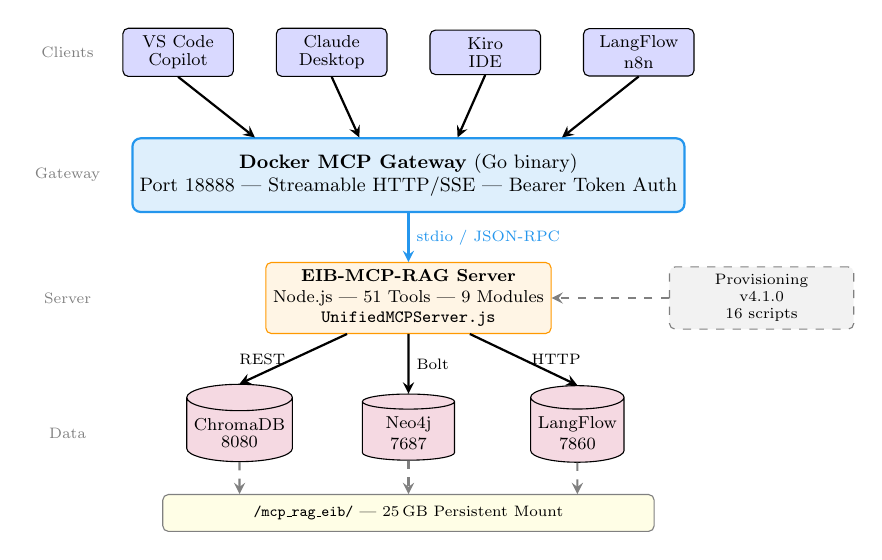
\begin{tikzpicture}[
    scale=0.78,
    every node/.style={transform shape},
    client/.style={rectangle, draw, fill=blue!15, minimum width=1.8cm,
                   minimum height=0.7cm, font=\footnotesize, rounded corners=2pt},
    gateway/.style={rectangle, draw=dockerblue, fill=dockerblue!15,
                   minimum width=8cm, minimum height=1.2cm, font=\small,
                   align=center, rounded corners=3pt, thick},
    server/.style={rectangle, draw=awsorange, fill=awsorange!10,
                  minimum width=3cm, minimum height=1cm, font=\footnotesize,
                  align=center, rounded corners=2pt},
    db/.style={cylinder, draw, fill=purple!15, minimum width=1.5cm,
              minimum height=0.9cm, font=\footnotesize, shape border rotate=90,
              aspect=0.25},
    provision/.style={rectangle, draw=gray, fill=gray!10, minimum width=3cm,
                     minimum height=0.7cm, font=\scriptsize, align=center,
                     rounded corners=2pt, dashed},
    arrow/.style={->, thick, >=stealth},
    label/.style={font=\scriptsize, gray}
]

% Clients
\node[client] at (0,7) (vscode) {\shortstack{VS Code\\Copilot}};
\node[client] at (2.5,7) (claude) {\shortstack{Claude\\Desktop}};
\node[client] at (5,7) (kiro) {\shortstack{Kiro\\IDE}};
\node[client] at (7.5,7) (langflow) {\shortstack{LangFlow\\n8n}};

% Gateway
\node[gateway] at (3.75,5) (gw) {\textbf{Docker MCP Gateway} (Go binary)\\
    Port 18888 --- Streamable HTTP/SSE --- Bearer Token Auth};

% MCP Server
\node[server] at (3.75,3) (mcp) {\textbf{EIB-MCP-RAG Server}\\
    Node.js --- 51 Tools --- 9 Modules\\
    \texttt{UnifiedMCPServer.js}};

% Databases
\node[db] at (1,0.8) (chromadb) {\shortstack{ChromaDB\\8080}};
\node[db] at (3.75,0.8) (neo4j) {\shortstack{Neo4j\\7687}};
\node[db] at (6.5,0.8) (langflowdb) {\shortstack{LangFlow\\7860}};

% Provisioning
\node[provision] at (9.5,3) (prov) {Provisioning\\v4.1.0\\16 scripts};

% Persistent storage
\node[rectangle, draw=gray, fill=yellow!10, minimum width=8cm,
      minimum height=0.6cm, font=\scriptsize, rounded corners=2pt]
      at (3.75,-0.5) (storage) {\texttt{/mcp\_rag\_eib/} --- 25\,GB Persistent Mount};

% Arrows
\draw[arrow] (vscode.south) -- ([xshift=-2.5cm]gw.north);
\draw[arrow] (claude.south) -- ([xshift=-0.8cm]gw.north);
\draw[arrow] (kiro.south) -- ([xshift=0.8cm]gw.north);
\draw[arrow] (langflow.south) -- ([xshift=2.5cm]gw.north);

\draw[arrow, dockerblue] (gw.south) -- node[right, font=\scriptsize] {stdio / JSON-RPC} (mcp.north);

\draw[arrow] ([xshift=-1cm]mcp.south) -- node[left, font=\scriptsize] {REST} (chromadb.north);
\draw[arrow] (mcp.south) -- node[right, font=\scriptsize] {Bolt} (neo4j.north);
\draw[arrow] ([xshift=1cm]mcp.south) -- node[right, font=\scriptsize] {HTTP} (langflowdb.north);

\draw[arrow, dashed, gray] (prov) -- (mcp);

\draw[arrow, gray, dashed] (chromadb.south) -- ([xshift=-2.75cm]storage.north);
\draw[arrow, gray, dashed] (neo4j.south) -- (storage.north);
\draw[arrow, gray, dashed] (langflowdb.south) -- ([xshift=2.75cm]storage.north);

% Layer labels
\node[label] at (-1.8,7) {Clients};
\node[label] at (-1.8,5) {Gateway};
\node[label] at (-1.8,3) {Server};
\node[label] at (-1.8,0.8) {Data};

\end{tikzpicture}
\caption{Legacy COTS architecture: Docker MCP Gateway bridging stdio to HTTP/SSE
for multi-client access to the containerized MCP server with ChromaDB and Neo4j backends.}
\label{fig:legacy-arch}
\end{figure}

\subsection{Component Inventory}

\begin{table}[H]
\centering
\footnotesize
\begin{tabular}{@{}llll@{}}
\toprule
\textbf{Component} & \textbf{Technology} & \textbf{Port} & \textbf{Data Scale} \\
\midrule
MCP Server & Node.js 20 & stdio & 51 tools, 9 modules \\
Vector DB & ChromaDB 0.5.x & 8080 & 85,921 docs, 768-dim \\
Graph DB & Neo4j 5 Community & 7687 & 95,565 nodes, 2.6M rels \\
Gateway & Docker MCP (Go) & 18888 & Streamable HTTP \\
Workflow UI & LangFlow / n8n & 7860 & Visual RAG pipelines \\
Provisioning & Bash (16 scripts) & --- & v4.1.0 modular \\
\bottomrule
\end{tabular}
\caption{Legacy component inventory.}
\label{tab:legacy-components}
\end{table}

\subsection{Docker MCP Gateway: Protocol Bridge}

The Docker MCP Gateway, an open-source Go binary from Docker Inc., solved
the fundamental MCP single-client limitation by bridging HTTP/SSE transport
to stdio-based MCP servers running in Docker containers. Key capabilities:

\begin{itemize}[noitemsep]
    \item \textbf{Container discovery} via \texttt{io.docker.server.metadata} Docker labels
    \item \textbf{Session management} with unique session IDs per client connection
    \item \textbf{Bearer token authentication} via \texttt{MCP\_GATEWAY\_AUTH\_TOKEN}
    \item \textbf{Resource limits} per container (CPU, memory constraints)
    \item \textbf{Network isolation} by default (containers cannot access host network)
\end{itemize}

A critical finding during deployment: the gateway's network isolation
prevented database connectivity. Our RAG server required ChromaDB and Neo4j
access, necessitating a ``gateway bypass'' pattern where the MCP container
ran on a shared Docker network with explicit database connectivity.

\subsection{Provisioning System}

The modular provisioning system (v4.1.0) comprised 16 independently
runnable scripts orchestrated by \texttt{provision.sh}:

\begin{lstlisting}[language=bash,caption={Provisioning script inventory (abbreviated).}]
00-users.sh          # Linux user accounts
01-directories.sh    # /mcp_rag_eib/ structure
02-system-deps.sh    # System packages
03-docker.sh         # Docker engine
04-nodejs.sh         # Node.js 20 LTS
05-python-spack.sh   # Python + Spack modules
06-chromadb.sh       # ChromaDB Docker container
07-mcp-server.sh     # MCP server deployment
08-services.sh       # Neo4j, n8n, systemd
11-docker-mcp-gateway.sh  # Go compiler + gateway build
12-static-mode-gateway.sh # Phase 23 static mode
13-container-cleanup.sh   # Smart cleanup timer
\end{lstlisting}

\subsection{Limitations Driving the AWS Port}

\begin{enumerate}[noitemsep]
    \item \textbf{Ephemeral VMs}: Parallel Works VMs are destroyed on session
          end; reprovisioning takes 15--20 minutes per startup.
    \item \textbf{Dev tunnel dependency}: Multi-client access required VS Code
          dev tunnels (\texttt{devtunnels.ms}), introducing external dependency
          and latency.
    \item \textbf{No auto-scaling}: Single container, single session at a time.
    \item \textbf{Security}: HTTP endpoint exposed via public dev tunnel URL.
    \item \textbf{Data durability}: 25\,GB persistent mount with no backup strategy.
\end{enumerate}

%===============================================================================
\section{AWS-Native Target Architecture}
\label{sec:aws-arch}
%===============================================================================

The AWS port replaces every COTS component with a managed equivalent while
preserving the 51-tool MCP interface. Figure~\ref{fig:aws-arch} shows the
complete target topology.

\begin{figure}[H]
\centering
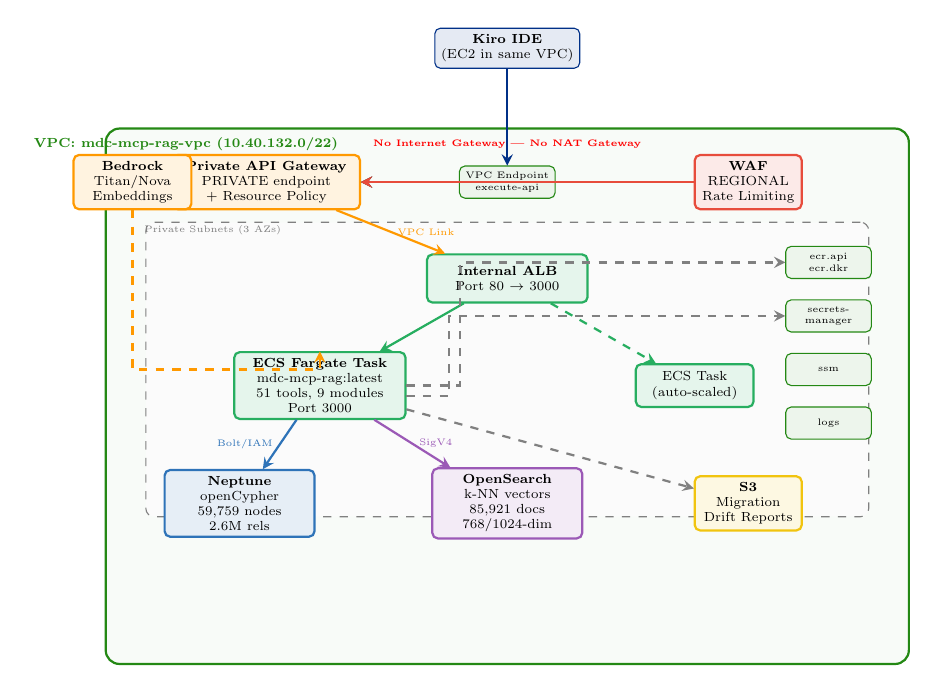
\begin{tikzpicture}[
    scale=0.68,
    every node/.style={transform shape},
    awsservice/.style={rectangle, draw=#1, fill=#1!12, minimum width=2.4cm,
                       minimum height=0.9cm, font=\scriptsize, align=center,
                       rounded corners=2pt, thick},
    awsservice/.default=awslightblue,
    vpce/.style={rectangle, draw=vpcgreen, fill=vpcgreen!8, minimum width=1.6cm,
                minimum height=0.6cm, font=\tiny, align=center, rounded corners=2pt},
    client/.style={rectangle, draw=noaablue, fill=noaablue!10, minimum width=2cm,
                  minimum height=0.7cm, font=\scriptsize, align=center, rounded corners=2pt},
    arrow/.style={->, thick, >=stealth},
    vpcbox/.style={draw=vpcgreen, thick, rounded corners=5pt, fill=vpcgreen!3},
    subnetbox/.style={draw=gray, dashed, rounded corners=3pt, fill=gray!3}
]

% VPC boundary
\node[vpcbox, minimum width=15cm, minimum height=10cm] at (7.5,4) (vpc) {};
\node[font=\scriptsize\bfseries, vpcgreen] at (1.5,8.7) {VPC: mdc-mcp-rag-vpc (10.40.132.0/22)};
\node[font=\tiny, red] at (7.5,8.7) {\textbf{No Internet Gateway --- No NAT Gateway}};

% Private subnets box
\node[subnetbox, minimum width=13.5cm, minimum height=5.5cm] at (7.5,4.5) {};
\node[font=\tiny, gray] at (2,7.1) {Private Subnets (3 AZs)};

% Client (outside VPC)
\node[client] at (7.5,10.5) (kiro) {\textbf{Kiro IDE}\\(EC2 in same VPC)};

% VPC Endpoint for API Gateway
\node[vpce] at (7.5,8) (vpce-exec) {VPC Endpoint\\execute-api};

% API Gateway (outside VPC logically)
\node[awsservice=awsorange, minimum width=3.5cm] at (3,8) (apigw)
    {\textbf{Private API Gateway}\\PRIVATE endpoint\\+ Resource Policy};

% WAF
\node[awsservice=cognitored, minimum width=2cm] at (12,8) (waf)
    {\textbf{WAF}\\REGIONAL\\Rate Limiting};

% ALB
\node[awsservice=ecsgreen, minimum width=3cm] at (7.5,6.2) (alb)
    {\textbf{Internal ALB}\\Port 80 $\rightarrow$ 3000};

% ECS Tasks
\node[awsservice=ecsgreen, minimum width=3.2cm, minimum height=1.2cm] at (4,4.2) (ecs1)
    {\textbf{ECS Fargate Task}\\mdc-mcp-rag:latest\\51 tools, 9 modules\\Port 3000};
\node[awsservice=ecsgreen, minimum width=2.2cm, minimum height=0.8cm] at (11,4.2) (ecs2)
    {ECS Task\\(auto-scaled)};

% Databases
\node[awsservice=neptuneblue, minimum width=2.8cm] at (2.5,2) (neptune)
    {\textbf{Neptune}\\openCypher\\59,759 nodes\\2.6M rels};
\node[awsservice=opensearchpurple, minimum width=2.8cm] at (7.5,2) (opensearch)
    {\textbf{OpenSearch}\\k-NN vectors\\85,921 docs\\768/1024-dim};
\node[awsservice=s3yellow, minimum width=2cm] at (12,2) (s3)
    {\textbf{S3}\\Migration\\Drift Reports};

% VPC Endpoints column
\node[vpce] at (13.5,6.5) (vpce-ecr) {ecr.api\\ecr.dkr};
\node[vpce] at (13.5,5.5) (vpce-sm) {secrets-\\manager};
\node[vpce] at (13.5,4.5) (vpce-ssm) {ssm};
\node[vpce] at (13.5,3.5) (vpce-logs) {logs};

% Arrows
\draw[arrow, noaablue] (kiro) -- (vpce-exec);
\draw[arrow] (vpce-exec) -- (apigw);
\draw[arrow, awsorange] (apigw) -- node[right, font=\tiny] {VPC Link} (alb);
\draw[arrow, cognitored] (waf) -- (apigw);

\draw[arrow, ecsgreen] (alb) -- (ecs1);
\draw[arrow, ecsgreen, dashed] (alb) -- (ecs2);

\draw[arrow, neptuneblue] (ecs1) -- node[left, font=\tiny] {Bolt/IAM} (neptune);
\draw[arrow, opensearchpurple] (ecs1) -- node[right, font=\tiny] {SigV4} (opensearch);
\draw[arrow, gray, dashed] (ecs1) -- (s3);

\draw[arrow, gray, dashed] (ecs1.east) -- ++(1,0) |- (vpce-ecr.west);
\draw[arrow, gray, dashed] ([yshift=-2mm]ecs1.east) -- ++(0.8,0) |- (vpce-sm.west);

% Bedrock (outside VPC)
\node[awsservice=awsorange, minimum width=2.2cm] at (0.5,8) (bedrock)
    {\textbf{Bedrock}\\Titan/Nova\\Embeddings};
\draw[arrow, dashed, awsorange] (bedrock) -- ++(0,-3.5) -| (ecs1);

\end{tikzpicture}
\caption{AWS-native target architecture: Private API Gateway with VPC-only access,
ECS Fargate hosting, Neptune graph database, and OpenSearch vector search.
No Internet Gateway exists in this VPC.}
\label{fig:aws-arch}
\end{figure}

\subsection{Component Mapping: Legacy to AWS}

\begin{table}[H]
\centering
\footnotesize
\begin{tabular}{@{}lll@{}}
\toprule
\textbf{Legacy Component} & \textbf{AWS Replacement} & \textbf{Benefit} \\
\midrule
ChromaDB (Docker) & Amazon OpenSearch (k-NN) & Managed, SigV4 auth, hybrid search \\
Neo4j (Docker) & Amazon Neptune & Managed, openCypher, IAM auth \\
Docker MCP Gateway & Private API Gateway & VPC-only, WAF, auto-scaling \\
MCP Server (Docker) & ECS Fargate & Serverless containers, ALB \\
Dev tunnel (HTTP) & VPC Endpoint & Zero internet exposure \\
\texttt{mcp-env.sh} & Secrets Manager + SSM & Encrypted, audited, rotatable \\
Docker Compose & AWS CDK (TypeScript) & Infrastructure as code, 4 stacks \\
Persistent mount & EFS + S3 & Durable, backed up, versioned \\
Manual provisioning & CDK deploy & Repeatable, 10-minute deploy \\
\bottomrule
\end{tabular}
\caption{Legacy to AWS component mapping.}
\label{tab:component-mapping}
\end{table}

\subsection{CDK Stack Decomposition}

The infrastructure is defined across four CDK stacks following AWS
best practices for separation of concerns:

\begin{table}[H]
\centering
\footnotesize
\begin{tabular}{@{}llll@{}}
\toprule
\textbf{Stack} & \textbf{Resources} & \textbf{Dependencies} & \textbf{Phase} \\
\midrule
\texttt{MdcVpcStack} & VPC, subnets, VPC endpoints & None & 48A \\
\texttt{MdcSecurityStack} & WAF, Secrets Manager, IAM & VpcStack & 48A \\
\texttt{MdcDataStack} & Neptune, OpenSearch, EFS, S3 & SecurityStack & 48C \\
\texttt{MdcServerStack} & ECS, ALB, API Gateway & All above & 48B \\
\bottomrule
\end{tabular}
\caption{CDK stack decomposition with dependency chain.}
\label{tab:cdk-stacks}
\end{table}

\subsection{Network Security: Zero Internet Exposure}

The VPC (\texttt{vpc-055f30ffa3d661e6b}) contains:
\begin{itemize}[noitemsep]
    \item 3 private subnets across 3 Availability Zones
    \item \textbf{No Internet Gateway} and \textbf{no NAT Gateway}
    \item 10 VPC endpoints for AWS service access (S3, ECR, Secrets Manager,
          SSM, CloudWatch Logs, execute-api, Neptune, OpenSearch, STS, Bedrock)
    \item API Gateway configured as \texttt{PRIVATE} endpoint type with a
          resource policy restricting access to the VPC endpoint
\end{itemize}

The Deny-first resource policy ensures that even if additional Allow
statements are added, requests not originating from the VPC endpoint are
always rejected:

\begin{lstlisting}[caption={API Gateway resource policy (Deny-first pattern).}]
{
  "Statement": [
    {
      "Effect": "Deny",
      "Principal": "*",
      "Action": "execute-api:Invoke",
      "Resource": "execute-api:/*",
      "Condition": {
        "StringNotEquals": {
          "aws:sourceVpce": "${vpce-id}"
        }
      }
    },
    {
      "Effect": "Allow",
      "Principal": "*",
      "Action": "execute-api:Invoke",
      "Resource": "execute-api:/*"
    }
  ]
}
\end{lstlisting}


%===============================================================================
\section{Adapter Pattern: Transparent Backend Switching}
\label{sec:adapter}
%===============================================================================

The critical design decision enabling the migration was the adapter pattern
in the data access layer. All 51 MCP tools interact with databases through
two abstract interfaces---\texttt{VectorDatabaseAdapter} and
\texttt{GraphDatabaseAdapter}---with concrete implementations for both
legacy and AWS backends.

\subsection{Interface Contracts}

\begin{figure}[H]
\centering
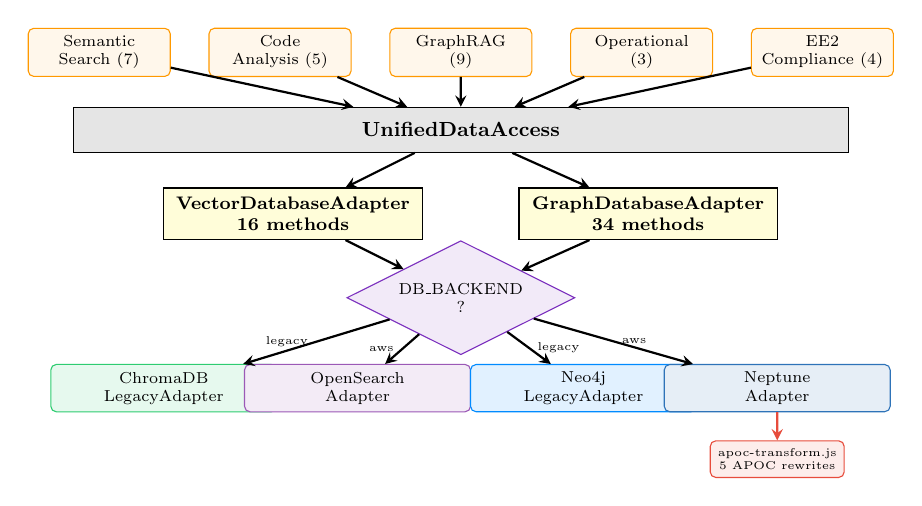
\begin{tikzpicture}[
    scale=0.82,
    every node/.style={transform shape},
    interface/.style={rectangle, draw=black, fill=yellow!15, minimum width=4cm,
                     minimum height=0.8cm, font=\footnotesize\bfseries, align=center},
    impl/.style={rectangle, draw=#1, fill=#1!12, minimum width=3.5cm,
                minimum height=0.7cm, font=\scriptsize, align=center, rounded corners=2pt},
    impl/.default=gray,
    tool/.style={rectangle, draw=awsorange, fill=awsorange!8, minimum width=2.2cm,
                minimum height=0.6cm, font=\scriptsize, align=center, rounded corners=2pt},
    selector/.style={diamond, draw=kiropurple, fill=kiropurple!10,
                    minimum width=1.5cm, minimum height=1cm, font=\scriptsize,
                    align=center, aspect=2},
    arrow/.style={->, thick, >=stealth}
]

% Tool modules (top)
\node[tool] at (0,6) (sst) {Semantic\\Search (7)};
\node[tool] at (2.8,6) (cat) {Code\\Analysis (5)};
\node[tool] at (5.6,6) (grt) {GraphRAG\\(9)};
\node[tool] at (8.4,6) (ot) {Operational\\(3)};
\node[tool] at (11.2,6) (ee2) {EE2\\Compliance (4)};

% UnifiedDataAccess
\node[rectangle, draw=black, fill=gray!20, minimum width=12cm,
      minimum height=0.7cm, font=\small\bfseries] at (5.6,4.8) (uda)
      {UnifiedDataAccess};

% Interfaces
\node[interface] at (3,3.5) (vda) {VectorDatabaseAdapter\\16 methods};
\node[interface] at (8.5,3.5) (gda) {GraphDatabaseAdapter\\34 methods};

% Backend selector
\node[selector] at (5.6,2.2) (bs) {DB\_BACKEND\\?};

% Implementations
\node[impl=chromagreen] at (1,0.8) (chroma) {ChromaDB\\LegacyAdapter};
\node[impl=opensearchpurple] at (4,0.8) (os) {OpenSearch\\Adapter};
\node[impl=neo4jgreen] at (7.5,0.8) (neo4j) {Neo4j\\LegacyAdapter};
\node[impl=neptuneblue] at (10.5,0.8) (neptune) {Neptune\\Adapter};

% APOC transform
\node[rectangle, draw=cognitored, fill=cognitored!10, minimum width=2cm,
      minimum height=0.5cm, font=\tiny, align=center, rounded corners=2pt]
      at (10.5,-0.3) (apoc) {apoc-transform.js\\5 APOC rewrites};

% Arrows from tools to UDA
\foreach \t in {sst, cat, grt, ot, ee2}
    \draw[arrow] (\t) -- (uda);

% UDA to interfaces
\draw[arrow] (uda) -- (vda);
\draw[arrow] (uda) -- (gda);

% Interfaces to selector
\draw[arrow] (vda) -- (bs);
\draw[arrow] (gda) -- (bs);

% Selector to implementations
\draw[arrow] (bs) -- node[left, font=\tiny] {legacy} (chroma);
\draw[arrow] (bs) -- node[left, font=\tiny] {aws} (os);
\draw[arrow] (bs) -- node[right, font=\tiny] {legacy} (neo4j);
\draw[arrow] (bs) -- node[right, font=\tiny] {aws} (neptune);

% Neptune to APOC
\draw[arrow, cognitored] (neptune) -- (apoc);

\end{tikzpicture}
\caption{Adapter pattern: \texttt{backend-selector.js} routes database calls
based on \texttt{DB\_BACKEND} environment variable. All 51 tools are unchanged.}
\label{fig:adapter-pattern}
\end{figure}

\subsection{Vector Database Adapter Interface}

\begin{lstlisting}[caption={VectorDatabaseAdapter interface (16 methods).}]
interface VectorDatabaseAdapter {
  connect(): Promise<void>
  query(collection, text, opts): Promise<QueryResult>
  multiCollectionQuery(collections[], text, opts): Promise<QueryResult>
  addDocuments(collection, docs[]): Promise<void>
  listCollections(): Promise<CollectionInfo[]>
  getCollectionCount(collection): Promise<number>
  healthCheck(opts): Promise<HealthStatus>
  close(): Promise<void>
  // + 8 additional methods for hybrid search, comparative query
}
\end{lstlisting}

\subsection{Graph Database Adapter Interface}

\begin{lstlisting}[caption={GraphDatabaseAdapter interface (34 methods).}]
interface GraphDatabaseAdapter {
  connect(): Promise<void>
  query(cypher, params): Promise<Record[]>
  findCallers(name): Promise<Node[]>
  traceCallChain(name, depth): Promise<Path[]>
  traceCrossLanguageChain(name, depth, direction): Promise<Chain[]>
  findUpstreamExecutors(name): Promise<Executor[]>
  getStatistics(): Promise<GraphStats>
  healthCheck(): Promise<HealthStatus>
  close(): Promise<void>
  // + 25 additional methods for graph traversal
}
\end{lstlisting}

\subsection{Backend Selection Algorithm}

\begin{algorithm}[H]
\caption{Database Backend Selection}
\label{alg:backend-select}
\begin{algorithmic}[1]
\REQUIRE $env \in \{development, devops, staging, production, aws\}$
\ENSURE Both adapters connected and healthy
\STATE $backend \gets$ SSM.getParameter(\texttt{/mdc-mcp-rag/db-backend}) $\lor$ $env$
\IF{$backend = $ \texttt{aws}}
    \STATE $vectorAdapter \gets$ new OpenSearchAdapter(SSM endpoint)
    \STATE $graphAdapter \gets$ new NeptuneAdapter(SSM endpoint)
\ELSIF{$backend = $ \texttt{legacy}}
    \STATE $vectorAdapter \gets$ new ChromaDBAdapter(env config)
    \STATE $graphAdapter \gets$ new Neo4jAdapter(env config)
\ELSE
    \STATE \textbf{error}(``Unknown backend: '' $\|$ $backend$)
\ENDIF
\STATE \textbf{await} $vectorAdapter$.connect()
\STATE \textbf{await} $graphAdapter$.connect()
\STATE \textbf{assert} $vectorAdapter$.healthCheck().status $=$ ``healthy''
\STATE \textbf{assert} $graphAdapter$.healthCheck().status $=$ ``healthy''
\RETURN $(vectorAdapter, graphAdapter)$
\end{algorithmic}
\end{algorithm}

\subsection{APOC Procedure Transformation Engine}

Neptune's openCypher implementation does not support Neo4j's APOC library.
The \texttt{apoc-transform.js} module intercepts Cypher queries containing
APOC calls and rewrites them to Neptune-compatible openCypher:

\begin{table}[H]
\centering
\footnotesize
\begin{tabular}{@{}lll@{}}
\toprule
\textbf{APOC Procedure} & \textbf{Neptune Replacement} & \textbf{Semantics} \\
\midrule
\texttt{apoc.path.expand} & Variable-length \texttt{MATCH} & Path traversal \\
\texttt{apoc.algo.dijkstra} & Multi-hop \texttt{MATCH} + cost & Shortest path \\
\texttt{apoc.periodic.iterate} & Batched \texttt{UNWIND} & Bulk operations \\
\texttt{apoc.create.node} & \texttt{CREATE} with labels & Node creation \\
\texttt{apoc.merge.node} & \texttt{MERGE} + \texttt{ON CREATE/MATCH SET} & Upsert \\
\bottomrule
\end{tabular}
\caption{APOC to openCypher transformation rules.}
\label{tab:apoc-transforms}
\end{table}

A critical Neptune compatibility issue discovered during validation:
Neptune rejects \textbf{directed variable-length path} syntax
(\texttt{-\relax[:REL*1..N]->}) that Neo4j supports. The fix decomposes these
into multiple \texttt{OPTIONAL MATCH} clauses per relationship type and
hop level, matching the pattern used by the legacy \texttt{GraphDatabase.js}.

%===============================================================================
\section{Data Migration: S3 Staging Pipeline}
\label{sec:migration}
%===============================================================================

The migration moved 85,921 vector documents and a 59,759-node / 2.6M-relationship
graph from Parallel Works VMs to AWS managed services via S3 staging.

\subsection{Migration Pipeline}

\begin{figure}[H]
\centering
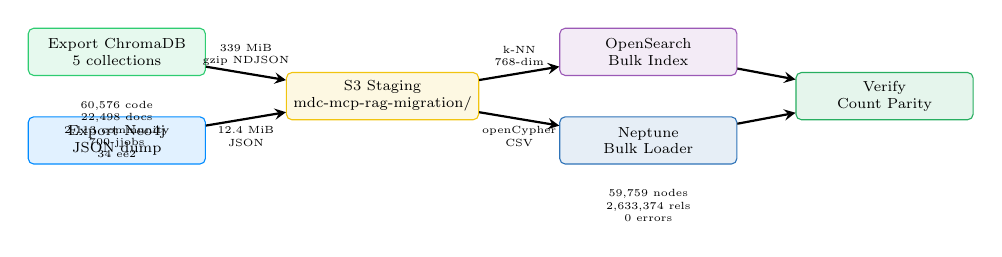
\begin{tikzpicture}[
    scale=0.75,
    every node/.style={transform shape},
    phase/.style={rectangle, draw=#1, fill=#1!12, minimum width=3cm,
                 minimum height=0.8cm, font=\scriptsize, align=center,
                 rounded corners=2pt},
    phase/.default=awslightblue,
    arrow/.style={->, thick, >=stealth},
    data/.style={font=\tiny, align=center}
]

% Phase 1: Export
\node[phase=chromagreen] at (0,4) (exp-v) {Export ChromaDB\\5 collections};
\node[phase=neo4jgreen] at (0,2.5) (exp-g) {Export Neo4j\\JSON dump};

% Phase 2: S3
\node[phase=s3yellow] at (4.5,3.25) (s3) {S3 Staging\\mdc-mcp-rag-migration/};

% Phase 3: Load
\node[phase=opensearchpurple] at (9,4) (load-v) {OpenSearch\\Bulk Index};
\node[phase=neptuneblue] at (9,2.5) (load-g) {Neptune\\Bulk Loader};

% Phase 4: Verify
\node[phase=ecsgreen] at (13,3.25) (verify) {Verify\\Count Parity};

% Arrows
\draw[arrow] (exp-v) -- node[above, data] {339 MiB\\gzip NDJSON} (s3);
\draw[arrow] (exp-g) -- node[below, data] {12.4 MiB\\JSON} (s3);
\draw[arrow] (s3) -- node[above, data] {k-NN\\768-dim} (load-v);
\draw[arrow] (s3) -- node[below, data] {openCypher\\CSV} (load-g);
\draw[arrow] (load-v) -- (verify);
\draw[arrow] (load-g) -- (verify);

% Data annotations
\node[data, below=0.3cm of exp-v] {60,576 code\\22,498 docs\\2,113 community\\700 jjobs\\34 ee2};
\node[data, below=0.3cm of load-g] {59,759 nodes\\2,633,374 rels\\0 errors};

\end{tikzpicture}
\caption{Four-phase migration pipeline via S3 staging.}
\label{fig:migration-pipeline}
\end{figure}

\subsection{Vector Migration: ChromaDB to OpenSearch}

\begin{table}[H]
\centering
\footnotesize
\begin{tabular}{@{}llrrl@{}}
\toprule
\textbf{ChromaDB Collection} & \textbf{OpenSearch Index} & \textbf{Docs} & \textbf{Size} & \textbf{Status} \\
\midrule
\texttt{code-with-context-v8-0-0} & \texttt{mdc-code-context-mpnet768} & 60,576 & 234 MiB & \checkmark \\
\texttt{global-workflow-docs-v8-0-0} & \texttt{mdc-workflow-docs-mpnet768} & 22,498 & 95 MiB & \checkmark \\
\texttt{community-summaries} & \texttt{mdc-community-summaries-mpnet768} & 2,113 & 8 MiB & \checkmark \\
\texttt{jjobs-v8-0-0} & \texttt{mdc-jjobs-mpnet768} & 700 & 3 MiB & \checkmark \\
\texttt{ee2-standards-v5-0-0-enhanced} & \texttt{mdc-ee2-standards-mpnet768} & 34 & 160 KiB & \checkmark \\
\midrule
\textbf{Total} & & \textbf{85,921} & \textbf{339 MiB} & \\
\bottomrule
\end{tabular}
\caption{ChromaDB to OpenSearch migration results.}
\label{tab:vector-migration}
\end{table}

\subsection{Graph Migration: Neo4j to Neptune}

The graph migration required two attempts. The initial Bolt-based approach
(\texttt{migrate-to-aws.js} Phase 50) silently failed---a \texttt{.catch()}
handler swallowed all relationship MERGE batch errors, wrote a false ``done''
watermark, and left Neptune with zero relationships despite reporting
2,633,374 loaded. This bug was identified and documented in Kiro Spec
\texttt{neptune-rel-load-fix}.

The remediation (Phase 50b) used Neptune's native bulk loader:

\begin{enumerate}[noitemsep]
    \item \textbf{Purge}: Batched \texttt{DETACH DELETE} of 45,296 orphan nodes
          from the crashed first run
    \item \textbf{Convert}: \texttt{convert-to-opencypher-csv.js} transformed
          the JSON dump to openCypher CSV with \texttt{label:name} composite
          node IDs (resolving cross-label collisions on names like
          \texttt{\_\_init\_\_} and \texttt{main})
    \item \textbf{Upload}: CSV files to \texttt{s3://mdc-mcp-rag-migration/}
    \item \textbf{Load}: Neptune \texttt{/loader} API with SigV4 auth---10--100x
          faster than Bolt, with internal parallelism
    \item \textbf{Verify}: Count parity check against legacy system
\end{enumerate}

\begin{table}[H]
\centering
\footnotesize
\begin{tabular}{@{}lrrl@{}}
\toprule
\textbf{Component} & \textbf{Legacy (PW)} & \textbf{AWS (Neptune)} & \textbf{Status} \\
\midrule
Nodes & 98,813 & 59,759 & \checkmark\ Deduplicated (39K dupes) \\
Relationships & 2,653,565 & 2,633,374 & \checkmark\ 99.2\% (20K unresolvable) \\
Node labels & 28 types & 28 types & \checkmark\ Exact match \\
Relationship types & 23 types & 23 types & \checkmark\ Exact match \\
\bottomrule
\end{tabular}
\caption{Graph migration parity results.}
\label{tab:graph-migration}
\end{table}


%===============================================================================
\section{Graph-Guided Semantic Retrieval (GGSR)}
\label{sec:ggsr}
%===============================================================================

The platform's distinguishing capability is Graph-Guided Semantic Retrieval
(GGSR)---a hybrid algorithm that fuses vector similarity search with
structural graph traversal to produce contextually rich results that
neither approach achieves alone.

\subsection{Algorithm Overview}

GGSR operates in three phases:

\begin{algorithm}[H]
\caption{Graph-Guided Semantic Retrieval}
\label{alg:ggsr}
\begin{algorithmic}[1]
\REQUIRE Query text $q$, knowledge graph $G = (V, E)$, vector index $I$
\ENSURE Ranked results with structural context
\STATE \textbf{Phase 1: Vector Seed}
\STATE $seeds \gets$ kNN$(I, \text{embed}(q), k=10)$ \COMMENT{OpenSearch k-NN}
\STATE \textbf{Phase 2: Graph Expansion}
\FOR{each $s \in seeds$}
    \STATE $N_1(s) \gets$ oneHopNeighborhood$(G, s)$ \COMMENT{Neptune openCypher}
    \STATE $N_2(s) \gets$ twoHopNeighborhood$(G, s)$ \COMMENT{Weighted traversal}
    \STATE $context(s) \gets N_1(s) \cup N_2(s)$
\ENDFOR
\STATE \textbf{Phase 3: Re-ranking}
\STATE $results \gets$ mergeAndRerank$(seeds, context, q)$
\RETURN $results$
\end{algorithmic}
\end{algorithm}

\subsection{Knowledge Graph Structure}

The knowledge graph contains 28 node types and 23 relationship types,
representing the complete structural decomposition of the Global Workflow
codebase:

\begin{figure}[H]
\centering
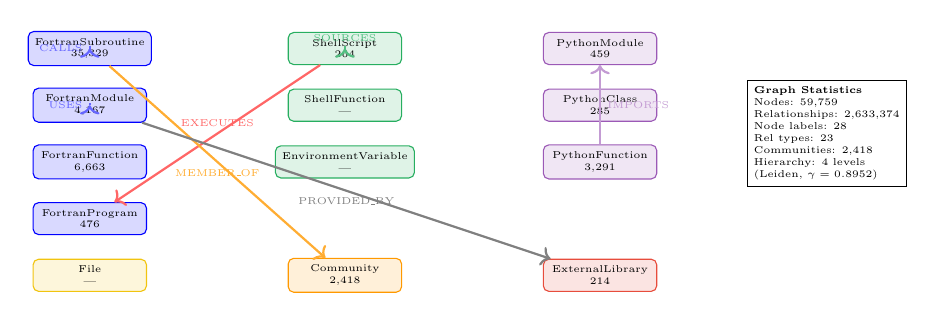
\begin{tikzpicture}[
    scale=0.72,
    every node/.style={transform shape},
    nodetype/.style={rectangle, draw=#1, fill=#1!15, minimum width=2cm,
                    minimum height=0.5cm, font=\tiny, align=center, rounded corners=2pt},
    nodetype/.default=gray,
    reltype/.style={font=\tiny, #1, align=center},
    reltype/.default=gray
]

% Fortran cluster
\node[nodetype=blue] at (0,4) (fsub) {FortranSubroutine\\35,329};
\node[nodetype=blue] at (0,3) (fmod) {FortranModule\\4,167};
\node[nodetype=blue] at (0,2) (ffun) {FortranFunction\\6,663};
\node[nodetype=blue] at (0,1) (fprog) {FortranProgram\\476};

% Shell cluster
\node[nodetype=ecsgreen] at (4.5,4) (shell) {ShellScript\\264};
\node[nodetype=ecsgreen] at (4.5,3) (sfun) {ShellFunction\\---};
\node[nodetype=ecsgreen] at (4.5,2) (env) {EnvironmentVariable\\---};

% Python cluster
\node[nodetype=opensearchpurple] at (9,4) (pymod) {PythonModule\\459};
\node[nodetype=opensearchpurple] at (9,3) (pycls) {PythonClass\\285};
\node[nodetype=opensearchpurple] at (9,2) (pyfun) {PythonFunction\\3,291};

% Infrastructure
\node[nodetype=awsorange] at (4.5,0) (comm) {Community\\2,418};
\node[nodetype=s3yellow] at (0,0) (file) {File\\---};
\node[nodetype=cognitored] at (9,0) (extlib) {ExternalLibrary\\214};

% Cross-language edges
\draw[->, thick, red!60] (shell) -- node[above, reltype=red!60] {EXECUTES} (fprog);
\draw[->, thick, blue!60] (fsub) -- node[left, reltype=blue!60] {CALLS} (fsub);
\draw[->, thick, blue!60] (fmod) -- node[left, reltype=blue!60] {USES} (fmod);
\draw[->, thick, ecsgreen!80] (shell) -- node[above, reltype=ecsgreen!80] {SOURCES} (shell);
\draw[->, thick, opensearchpurple!60] (pyfun) -- node[right, reltype=opensearchpurple!60] {IMPORTS} (pymod);
\draw[->, thick, awsorange!80] (fsub) -- node[below, reltype=awsorange!80] {MEMBER\_OF} (comm);
\draw[->, thick, gray] (fmod) -- node[below, reltype] {PROVIDED\_BY} (extlib);

% Stats box
\node[rectangle, draw=black, fill=white, font=\tiny, align=left] at (13,2.5) {
    \textbf{Graph Statistics}\\
    Nodes: 59,759\\
    Relationships: 2,633,374\\
    Node labels: 28\\
    Rel types: 23\\
    Communities: 2,418\\
    Hierarchy: 4 levels\\
    (Leiden, $\gamma=0.8952$)
};

\end{tikzpicture}
\caption{Knowledge graph schema showing major node types with counts and
cross-language relationship types.}
\label{fig:graph-schema}
\end{figure}

\subsection{GGSR Traversal Weights}

The GGSR traversal uses weighted edges to prioritize structurally
significant relationships:

\begin{table}[H]
\centering
\footnotesize
\begin{tabular}{@{}llr@{}}
\toprule
\textbf{Relationship} & \textbf{Semantics} & \textbf{Weight} \\
\midrule
CALLS & Direct function invocation & 1.0 \\
USES & Module dependency & 0.9 \\
CONTAINS & Parent-child containment & 0.8 \\
IMPORTS & Python import & 0.8 \\
EXECUTES & Shell $\rightarrow$ Fortran bridge & 0.7 \\
SOURCES & Shell script sourcing & 0.7 \\
PROVIDED\_BY & NCEPLIBS library link & 0.6 \\
TRANSITIVELY\_DEPENDS & Transitive library dep & 0.5 \\
DOCUMENTED\_BY & ChromaDB doc link & 0.4 \\
REQUIRES\_VERSION & Platform version pin & 0.3 \\
MEMBER\_OF & Community membership & 0.2 \\
\bottomrule
\end{tabular}
\caption{GGSR edge weights for graph-guided traversal.}
\label{tab:ggsr-weights}
\end{table}

\subsection{Hierarchical Community Detection}

The Leiden algorithm (GDS 2.13.7) partitions the graph into hierarchical
communities materialized as first-class Neo4j/Neptune entities:

\begin{itemize}[noitemsep]
    \item \textbf{4 hierarchy levels}: L0 (694 communities), L1 (175),
          L2 (86), L3 (81)
    \item \textbf{2,418 Community nodes} with LLM-generated summaries
          (820 via GitHub Models API using 10-model rotation)
    \item \textbf{73,086 MEMBER\_OF} relationships linking code entities
          to communities
    \item \textbf{1,655 PARENT\_OF} relationships forming the hierarchy tree
    \item \textbf{4,630 INTERACTS\_WITH} edges capturing cross-community
          coupling (avg strength: 69.7)
    \item Modularity score: 0.8952
\end{itemize}

%===============================================================================
\section{Multi-Model Embedding Pipeline}
\label{sec:embeddings}
%===============================================================================

Phase 49 restructured the ingestion pipeline from 14 independent scripts
with hardcoded embedding models into a modular, multi-model, registry-driven
architecture.

\subsection{Embedding Model Registry}

\begin{table}[H]
\centering
\footnotesize
\begin{tabular}{@{}llrlcc@{}}
\toprule
\textbf{Short Name} & \textbf{Provider} & \textbf{Dim} & \textbf{Model ID} & \textbf{Matryoshka} & \textbf{Multimodal} \\
\midrule
\texttt{mpnet768} & Local & 768 & all-mpnet-base-v2 & No & No \\
\texttt{titan1024} & Bedrock & 1024 & amazon.titan-embed-text-v2:0 & No & No \\
\texttt{nova256} & Bedrock & 256 & amazon.nova-2-multimodal-embed-v1:0 & Yes & Yes \\
\texttt{nova512} & Bedrock & 512 & amazon.nova-2-multimodal-embed-v1:0 & Yes & Yes \\
\texttt{nova1024} & Bedrock & 1024 & amazon.nova-2-multimodal-embed-v1:0 & Yes & Yes \\
\texttt{nova3072} & Bedrock & 3072 & amazon.nova-2-multimodal-embed-v1:0 & Yes & Yes \\
\bottomrule
\end{tabular}
\caption{Embedding model registry with 6 built-in profiles.}
\label{tab:embedding-models}
\end{table}

\subsection{Model-Aware Collection Naming}

Collections follow the pattern \texttt{\{domain\}-\{version\}-\{model\_short\}},
enabling multiple vector spaces for the same content domain to coexist:

\begin{lstlisting}[caption={Model-aware index naming examples.}]
mdc-code-context-mpnet768      # 60,576 docs, 768-dim
mdc-code-context-titan1024     # 58,961 docs, 1024-dim
mdc-workflow-docs-nova1024     # 150 docs (test), 1024-dim
\end{lstlisting}

\subsection{Hybrid Search: BM25 + Vector + RRF Fusion}

The \texttt{HybridSearchBuilder} constructs OpenSearch queries that combine
lexical (BM25) and semantic (k-NN) search with Reciprocal Rank Fusion:

\begin{algorithm}[H]
\caption{Hybrid Search with Code Identifier Detection}
\label{alg:hybrid-search}
\begin{algorithmic}[1]
\REQUIRE Query text $q$, embedding vector $\vec{v}$, search mode $m$
\ENSURE Ranked results with fused scores
\IF{$m = $ \texttt{hybrid}}
    \STATE $bm25\_weight \gets 1.0$
    \IF{containsCodeIdentifiers($q$)}
        \STATE $bm25\_weight \gets 2.0$ \COMMENT{Boost for camelCase, snake\_case, paths}
    \ENDIF
    \STATE $query \gets$ \{bool: \{must: [knn($\vec{v}$, $k$)], should: [match($q$, $bm25\_weight$)]\}\}
\ELSIF{$m = $ \texttt{vector}}
    \STATE $query \gets$ \{knn: \{embedding: \{vector: $\vec{v}$, k: $k$\}\}\}
\ELSIF{$m = $ \texttt{keyword}}
    \STATE $query \gets$ \{match: \{content: $q$\}\}
\ENDIF
\RETURN OpenSearch.search($query$)
\end{algorithmic}
\end{algorithm}

\subsection{Benchmark Results: Titan1024 vs MPNet768}

Phase 52 benchmarked the Bedrock Titan V2 embeddings against the local
MPNet baseline across 24 ground-truth queries:

\begin{table}[H]
\centering
\footnotesize
\begin{tabular}{@{}lrrrr@{}}
\toprule
\textbf{Model + Mode} & \textbf{P@5} & \textbf{P@10} & \textbf{MRR} & \textbf{nDCG} \\
\midrule
titan1024-hybrid & 0.267 & 0.196 & 0.511 & 0.536 \\
titan1024-vector & 0.158 & --- & 0.286 & --- \\
\bottomrule
\end{tabular}
\caption{Bedrock Titan1024 benchmark results. Hybrid search significantly
outperforms vector-only, validating the BM25+vector fusion approach.}
\label{tab:benchmark}
\end{table}

%===============================================================================
\section{Private MCP Deployment}
\label{sec:private}
%===============================================================================

The production deployment eliminates all internet-facing components. Kiro
connects to the MCP server through a Private API Gateway accessible only
via VPC endpoint.

\subsection{Request Flow}

\begin{enumerate}[noitemsep]
    \item Kiro MCP client sends HTTPS POST to
          \texttt{https://\{api-id\}-\{vpce-id\}.execute-api.\allowbreak us-east-1.amazonaws.com/prod/mcp}
    \item Request enters VPC through the \texttt{execute-api} VPC endpoint
    \item Private API Gateway validates against resource policy (must originate
          from VPC endpoint)
    \item WAF (REGIONAL scope) applies rate limiting and managed rules
    \item API Gateway proxies to Internal ALB via VPC Link
    \item ALB routes to a healthy ECS Fargate task
    \item ECS task processes the MCP request using Neptune (graph) and
          OpenSearch (vectors)
    \item Response returns through the same path
\end{enumerate}

\subsection{ECS Task Definition}

\begin{table}[H]
\centering
\footnotesize
\begin{tabular}{@{}ll@{}}
\toprule
\textbf{Property} & \textbf{Value} \\
\midrule
Family & \texttt{mdc-mcp-rag} \\
CPU / Memory & 1 vCPU / 2048 MiB \\
Network Mode & awsvpc \\
Container Port & 3000 \\
Image & \texttt{903050880929.dkr.ecr.us-east-1.amazonaws.com/mdc-mcp-rag:latest} \\
Task Role & \texttt{mdc-mcp-rag-ecs-task-role} \\
Execution Role & \texttt{mdc-mcp-rag-ecs-execution-role} \\
Environment & \texttt{DB\_BACKEND=aws}, \texttt{NODE\_ENV=production} \\
Health Check & \texttt{/health} $\rightarrow$ 200 \\
Auto-scaling & 1--4 tasks, scale on request count \\
\bottomrule
\end{tabular}
\caption{ECS Fargate task definition.}
\label{tab:ecs-task}
\end{table}

\subsection{IAM Least-Privilege Model}

Both ECS roles follow strict least-privilege:

\begin{itemize}[noitemsep]
    \item \textbf{Task role}: Read-only Secrets Manager + SSM, Neptune
          \texttt{connect}, OpenSearch HTTP operations---scoped to
          \texttt{mdc-mcp-rag/*} resources only
    \item \textbf{Execution role}: AWS managed policy for ECS task execution
          (ECR pull + CloudWatch Logs)
    \item Neither role grants internet access, S3 write, or IAM modification
    \item Both roles can only be assumed by \texttt{ecs-tasks.amazonaws.com}
\end{itemize}

\subsection{What Was Removed}

The private deployment eliminated several components from the initial
AWS design:

\begin{table}[H]
\centering
\footnotesize
\begin{tabular}{@{}lll@{}}
\toprule
\textbf{Component} & \textbf{Initial Design} & \textbf{Private Deployment} \\
\midrule
CloudFront Distribution & Yes (HTTPS, caching) & Removed \\
CLOUDFRONT WAF & Yes & Removed \\
API Gateway type & REGIONAL & PRIVATE \\
Authentication & Cognito User Pools & Resource Policy (VPC) \\
Cognito User Pool & Created & Removed \\
WAF scope & CLOUDFRONT + REGIONAL & REGIONAL only \\
Public endpoint & CloudFront domain & None \\
\bottomrule
\end{tabular}
\caption{Components removed in the private deployment.}
\label{tab:removed-components}
\end{table}


%===============================================================================
\section{Kiro Spec-Driven Development Methodology}
\label{sec:kiro}
%===============================================================================

The entire 52-phase evolution of this platform was governed by the
Spec-Driven Development (SDD) methodology, executed through Kiro's
specification system. SDD formalizes the design-implement-validate cycle
into machine-trackable artifacts.

\subsection{SDD Lifecycle}

\begin{figure}[H]
\centering
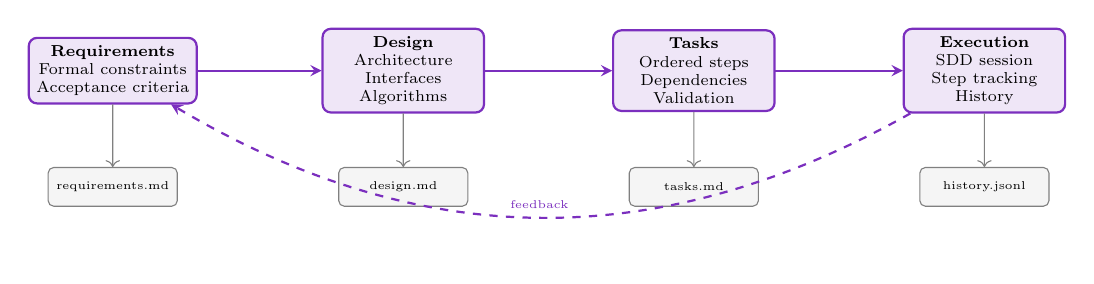
\begin{tikzpicture}[
    scale=0.82,
    every node/.style={transform shape},
    phase/.style={rectangle, draw=kiropurple, fill=kiropurple!12,
                 minimum width=2.5cm, minimum height=1cm, font=\scriptsize,
                 align=center, rounded corners=3pt, thick},
    artifact/.style={rectangle, draw=gray, fill=gray!8, minimum width=2cm,
                    minimum height=0.6cm, font=\tiny, align=center,
                    rounded corners=2pt},
    arrow/.style={->, thick, >=stealth, kiropurple}
]

% Phases
\node[phase] at (0,0) (req) {\textbf{Requirements}\\Formal constraints\\Acceptance criteria};
\node[phase] at (4.5,0) (design) {\textbf{Design}\\Architecture\\Interfaces\\Algorithms};
\node[phase] at (9,0) (tasks) {\textbf{Tasks}\\Ordered steps\\Dependencies\\Validation};
\node[phase] at (13.5,0) (exec) {\textbf{Execution}\\SDD session\\Step tracking\\History};

% Artifacts
\node[artifact] at (0,-1.8) (req-a) {requirements.md};
\node[artifact] at (4.5,-1.8) (des-a) {design.md};
\node[artifact] at (9,-1.8) (task-a) {tasks.md};
\node[artifact] at (13.5,-1.8) (hist-a) {history.jsonl};

% Arrows
\draw[arrow] (req) -- (design);
\draw[arrow] (design) -- (tasks);
\draw[arrow] (tasks) -- (exec);
\draw[arrow, dashed] (exec) to[bend left=30] node[above, font=\tiny, kiropurple] {feedback} (req);

\draw[->, gray] (req) -- (req-a);
\draw[->, gray] (design) -- (des-a);
\draw[->, gray] (tasks) -- (task-a);
\draw[->, gray] (exec) -- (hist-a);

\end{tikzpicture}
\caption{Kiro Spec-Driven Development lifecycle: requirements $\rightarrow$
design $\rightarrow$ tasks $\rightarrow$ execution with feedback loop.}
\label{fig:sdd-lifecycle}
\end{figure}

\subsection{Kiro Specifications for the AWS Port}

Seven formal specifications governed the AWS migration:

\begin{table}[H]
\centering
\footnotesize
\begin{tabular}{@{}lllr@{}}
\toprule
\textbf{Spec Name} & \textbf{Phase} & \textbf{Scope} & \textbf{Design Lines} \\
\midrule
\texttt{aws-infrastructure-port} & 48 & CDK stacks, adapters, migration & 922 \\
\texttt{aws-mcp-server-validation} & 48E & 51-tool validation, APOC PBT & 450 \\
\texttt{ingestion-pipeline-restructure} & 49 & Multi-model embeddings, registry & 680 \\
\texttt{bedrock-embedding-reingestion} & 52 & Titan1024 re-ingestion, benchmarks & 380 \\
\texttt{neptune-ggsr-compatibility} & 8.4 & Neptune VLP syntax, HTTP GGSR & 520 \\
\texttt{neptune-rel-load-fix} & 50b & Bulk loader, watermark fix & 490 \\
\texttt{private-mcp-deployment} & --- & Private API GW, no CloudFront & 610 \\
\bottomrule
\end{tabular}
\caption{Kiro specifications governing the AWS migration.}
\label{tab:kiro-specs}
\end{table}

\subsection{SDD MCP Tools}

The SDD framework is itself exposed as 9 MCP tools, enabling AI assistants
to participate in the development lifecycle:

\begin{table}[H]
\centering
\footnotesize
\begin{tabular}{@{}ll@{}}
\toprule
\textbf{Tool} & \textbf{Purpose} \\
\midrule
\texttt{list\_sdd\_workflows} & Enumerate available workflow specifications \\
\texttt{get\_sdd\_workflow} & Retrieve workflow details and steps \\
\texttt{start\_sdd\_session} & Begin a tracked development session \\
\texttt{record\_sdd\_step} & Log step completion with artifacts \\
\texttt{get\_sdd\_session} & Resume an in-progress session \\
\texttt{complete\_sdd\_session} & Finalize session with summary \\
\texttt{get\_sdd\_execution\_history} & View history with analytics \\
\texttt{validate\_sdd\_compliance} & Validate code against SDD standards \\
\texttt{get\_sdd\_framework\_status} & Framework health and metrics \\
\bottomrule
\end{tabular}
\caption{SDD MCP tools enabling AI-assisted development lifecycle management.}
\label{tab:sdd-tools}
\end{table}

\subsection{Property-Based Testing in Specifications}

Each Kiro specification includes formal correctness properties validated
through property-based testing (PBT) using \texttt{fast-check}. Example
properties from the AWS port:

\begin{enumerate}[noitemsep]
    \item \textbf{P1 Tool Interface Preservation}: For all 51 tools, the
          response schema is identical regardless of \texttt{DB\_BACKEND}
    \item \textbf{P3 APOC Semantic Preservation}: For any Cypher query
          containing a supported APOC call, the transformed openCypher
          produces equivalent results
    \item \textbf{P7 Score Normalization}: For all OpenSearch results,
          scores are normalized to $[0, 1]$
    \item \textbf{P11 Secret Non-Exposure}: For all log output and error
          messages, no secret values appear in plaintext
\end{enumerate}

%===============================================================================
\section{Advanced Capabilities on the Horizon}
\label{sec:advanced}
%===============================================================================

The Kiro specifications define several advanced capabilities currently in
development or planned for near-term implementation.

\subsection{Matryoshka Adaptive-Dimension Embeddings}

Amazon Nova Multimodal Embeddings support Matryoshka representation
learning, enabling queries at multiple dimension levels from a single
embedding:

\begin{figure}[H]
\centering
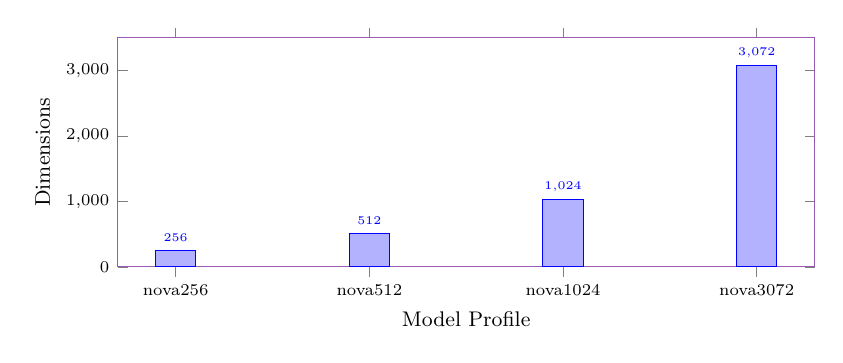
\begin{tikzpicture}[
    scale=0.85,
    every node/.style={transform shape}
]
\begin{axis}[
    ybar,
    bar width=0.6cm,
    width=12cm,
    height=5cm,
    ylabel={Dimensions},
    symbolic x coords={nova256, nova512, nova1024, nova3072},
    xtick=data,
    ymin=0,
    ymax=3500,
    nodes near coords,
    nodes near coords style={font=\tiny},
    xlabel={Model Profile},
    ylabel style={font=\small},
    xlabel style={font=\small},
    tick label style={font=\scriptsize},
    legend style={font=\tiny, at={(0.98,0.95)}, anchor=north east},
    fill=opensearchpurple!60,
    draw=opensearchpurple
]
\addplot coordinates {(nova256,256) (nova512,512) (nova1024,1024) (nova3072,3072)};
\end{axis}
\end{tikzpicture}
\caption{Nova Matryoshka embedding dimensions. A single 3072-dim embedding
can be truncated to 256, 512, or 1024 dimensions at query time with
100\% result overlap on test queries.}
\label{fig:matryoshka}
\end{figure}

The \texttt{MatryoshkaQuery} module truncates query vectors to a specified
prefix dimension and uses \texttt{script\_score} cosine similarity for
lower-dimension searches. Phase 52 testing confirmed 100\% result overlap
between 256-dim and 1024-dim queries on a 150-document test set.

\subsection{Self-Improving Retrieval Loop}

The ingestion pipeline restructure (Spec: \texttt{ingestion-pipeline-restructure})
defines a closed-loop quality improvement system:

\begin{figure}[H]
\centering
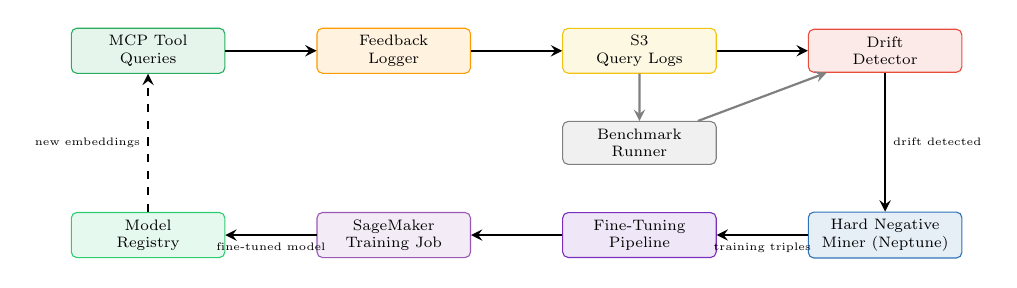
\begin{tikzpicture}[
    scale=0.78,
    every node/.style={transform shape},
    component/.style={rectangle, draw=#1, fill=#1!12, minimum width=2.5cm,
                     minimum height=0.7cm, font=\scriptsize, align=center,
                     rounded corners=2pt},
    component/.default=awslightblue,
    arrow/.style={->, thick, >=stealth}
]

% Components
\node[component=ecsgreen] at (0,3) (query) {MCP Tool\\Queries};
\node[component=awsorange] at (4,3) (feedback) {Feedback\\Logger};
\node[component=s3yellow] at (8,3) (s3) {S3\\Query Logs};
\node[component=cognitored] at (12,3) (drift) {Drift\\Detector};

\node[component=neptuneblue] at (12,0) (miner) {Hard Negative\\Miner (Neptune)};
\node[component=kiropurple] at (8,0) (finetune) {Fine-Tuning\\Pipeline};
\node[component=opensearchpurple] at (4,0) (sagemaker) {SageMaker\\Training Job};
\node[component=chromagreen] at (0,0) (registry) {Model\\Registry};

% Arrows
\draw[arrow] (query) -- (feedback);
\draw[arrow] (feedback) -- (s3);
\draw[arrow] (s3) -- (drift);
\draw[arrow] (drift) -- node[right, font=\tiny] {drift detected} (miner);
\draw[arrow] (miner) -- node[below, font=\tiny] {training triples} (finetune);
\draw[arrow] (finetune) -- (sagemaker);
\draw[arrow] (sagemaker) -- node[below, font=\tiny] {fine-tuned model} (registry);
\draw[arrow, dashed] (registry) -- node[left, font=\tiny] {new embeddings} (query);

% Benchmark
\node[component=gray] at (8,1.5) (bench) {Benchmark\\Runner};
\draw[arrow, gray] (bench) -- (drift);
\draw[arrow, gray] (s3) -- (bench);

\end{tikzpicture}
\caption{Self-improving retrieval loop: query feedback $\rightarrow$ drift
detection $\rightarrow$ graph-powered hard negative mining $\rightarrow$
domain-adaptive fine-tuning $\rightarrow$ model registry update.}
\label{fig:self-improving}
\end{figure}

Key components:

\begin{itemize}[noitemsep]
    \item \textbf{FeedbackLogger}: Anonymized query-result pair logging to S3
          (JSON Lines, no PII)
    \item \textbf{DriftDetector}: Samples $N$ documents, re-embeds with current
          model, computes cosine similarity; triggers re-ingestion when
          mean similarity drops below 0.95
    \item \textbf{HardNegativeMiner}: Uses Neptune graph structure to generate
          training triples---entity pairs that are 1-hop apart in the graph
          but belong to different functional domains
    \item \textbf{FineTuningPipeline}: Domain-adaptive fine-tuning using
          Sentence Transformers v3+ Trainer on SageMaker Training Jobs
    \item \textbf{BenchmarkRunner}: Precision@$k$, Recall@$k$, MRR, nDCG
          evaluation across models, dimensions, and search modes
\end{itemize}

\subsection{SageMaker Compute Offloading}

The \texttt{SageMakerJobLauncher} submits ingestion scripts as SageMaker
Processing Jobs, keeping the development EC2 free while running
GPU-accelerated embedding generation:

\begin{lstlisting}[caption={SageMaker job submission for embedding generation.}]
python3 sagemaker_launcher.py \
    ingest_code_v8.py \
    --model titan1024 \
    --backend aws \
    --instance-type ml.g5.xlarge \
    --dry-run  # estimate cost first
\end{lstlisting}

\subsection{Graph-Augmented Retrieval}

The \texttt{GraphAugmenter} module expands vector search results with
1-hop graph neighbors from Neptune, adding structural context that pure
vector search misses:

\begin{algorithm}[H]
\caption{Graph-Augmented Retrieval}
\label{alg:graph-augment}
\begin{algorithmic}[1]
\REQUIRE Vector results $R$, graph $G$, hop depth $d$
\ENSURE Results enriched with graph context
\FOR{each result $r \in R$}
    \STATE $entity \gets$ matchGraphEntity($r$.source\_file, $G$)
    \IF{$entity \neq \emptyset$}
        \STATE $neighbors \gets$ Neptune.query(
            ``MATCH ($entity$)-[:CALLS|USES|IMPORTS|CONTAINS*1..$d$]-(n) RETURN n'')
        \STATE $r$.graph\_context $\gets$ formatNeighbors($neighbors$)
    \ENDIF
\ENDFOR
\RETURN $R$
\end{algorithmic}
\end{algorithm}

\subsection{Comparative Multi-Model Queries}

The \texttt{comparativeQuery()} method on \texttt{VectorDatabaseAdapter}
enables A/B retrieval comparisons across embedding models:

\begin{lstlisting}[caption={Comparative query across embedding models.}]
// Query same content across mpnet768 and titan1024
const results = await dataAccess.comparativeQuery(
    "data assimilation initialization",
    ["mdc-code-context-mpnet768", "mdc-code-context-titan1024"],
    { k: 10, search_mode: "hybrid" }
);
// Returns results grouped by model profile
\end{lstlisting}

%===============================================================================
\section{Validation Results}
\label{sec:validation}
%===============================================================================

\subsection{Tool-by-Tool Validation}

The validation script (\texttt{validate-aws-mcp.js}) tested all 51 tools
against live AWS backends:

\begin{table}[H]
\centering
\footnotesize
\begin{tabular}{@{}lrrrr@{}}
\toprule
\textbf{Module} & \textbf{Total} & \textbf{Pass} & \textbf{Fail} & \textbf{Skip} \\
\midrule
WorkflowInfoTools & 3 & 3 & 0 & 0 \\
SemanticSearchTools & 7 & 7 & 0 & 0 \\
CodeAnalysisTools & 5 & 5 & 0 & 0 \\
GraphRAGTools & 9 & 9 & 0 & 0 \\
OperationalTools & 3 & 3 & 0 & 0 \\
EE2ComplianceTools & 4 & 4 & 0 & 0 \\
SDDWorkflowTools & 9 & 9 & 0 & 0 \\
UtilityTools & 5 & 5 & 0 & 0 \\
GitHubTools & 6 & --- & --- & 6 \\
\midrule
\textbf{Total} & \textbf{51} & \textbf{45} & \textbf{0} & \textbf{6} \\
\bottomrule
\end{tabular}
\caption{Tool validation results: 45/45 non-GitHub tools pass with
\texttt{DB\_BACKEND=aws}. GitHub tools skipped (external API, rate limits).}
\label{tab:validation}
\end{table}

\subsection{Performance Metrics}

\begin{table}[H]
\centering
\footnotesize
\begin{tabular}{@{}lr@{}}
\toprule
\textbf{Metric} & \textbf{Value} \\
\midrule
Server startup time & 706 ms (was 70+ seconds before shared instance fix) \\
Tool P50 latency & 7 ms \\
Tool P95 latency & 9,155 ms \\
Tool average latency & 686 ms \\
Hybrid search P50 & 117 ms \\
\bottomrule
\end{tabular}
\caption{Performance metrics on AWS backends.}
\label{tab:performance}
\end{table}

\subsection{Error Handling and Resilience}

The validation confirmed 9 error-handling scenarios:

\begin{itemize}[noitemsep]
    \item Server starts with bad Neptune endpoint; vector queries still work
    \item Neptune connection retries 4 times with exponential backoff
          (5s, 10s, 20s, 60s)
    \item OpenSearch SigV4 token refresh on expiry
    \item Per-tool timeout (30s default) with graceful error reporting
    \item Partial degradation: graph-down $\rightarrow$ vector tools pass;
          vector-down $\rightarrow$ graph tools pass
    \item Static tools (WorkflowInfo, SDD) always run regardless of backend
\end{itemize}

%===============================================================================
\section{Lessons Learned}
\label{sec:lessons}
%===============================================================================

\subsection{Neptune openCypher Compatibility}

Neptune's openCypher implementation differs from Neo4j in several ways
discovered during validation:

\begin{enumerate}[noitemsep]
    \item \textbf{Directed variable-length paths} (\texttt{->[:REL*1..N]->})
          are rejected; decompose into multiple \texttt{OPTIONAL MATCH} clauses
    \item \textbf{Multi-relationship VLP} (\texttt{[:A|B|C*1..N]}) may fail;
          use separate matches per relationship type
    \item \textbf{\texttt{labels(n)[0]}} is unreliable; use \texttt{head(labels(n))}
    \item \textbf{\texttt{length(path)}} unsupported; use \texttt{size(nodes(path))-1}
    \item \textbf{\texttt{=\~{}} regex operator} unsupported; use
          \texttt{toLower(x) CONTAINS toLower(y)}
    \item \textbf{APOC procedures} completely absent; requires pre-transform layer
    \item \textbf{Multi-label OR syntax} (\texttt{f:A|B|C}) unsupported; use
          \texttt{WHERE f:A OR f:B OR f:C}
\end{enumerate}

\subsection{Silent Failure Patterns}

The Neptune bulk load failure (Phase 50) revealed a dangerous pattern:
\texttt{.catch()} handlers that swallow errors in batch loops can write
false success watermarks. The fix: replace \texttt{.catch()} with error
accumulation and conditional watermark writing.

\subsection{IAM Role Creation in Restricted Environments}

NOAA's AWS account uses \texttt{PowerUserRestrictions} that deny
\texttt{iam:CreateRole}. CDK deployments fail when stacks attempt to
create IAM roles. The workaround: pre-create roles via admin request
documents and import them in CDK using \texttt{fromRoleName()}.

\subsection{VPC Endpoint Requirements}

A VPC with no Internet Gateway requires VPC endpoints for every AWS
service the application touches. Our deployment required 10 endpoints:
S3 (Gateway), ECR API, ECR DKR, Secrets Manager, SSM, CloudWatch Logs,
execute-api, Neptune, OpenSearch, and STS.

\subsection{Docker CE vs Docker Desktop}

The Docker MCP Gateway plugin initially only worked with Docker Desktop.
Pull Request \#301 (merged December 12, 2025) added Docker CE support.
Building from source after this merge is required for server deployments.

%===============================================================================
\section{Conclusion}
%===============================================================================

We have presented the complete port of the MDC MCP/RAG Server from a
Docker Compose stack to AWS-native managed services, achieving:

\begin{itemize}[noitemsep]
    \item \textbf{Zero tool changes}: All 51 MCP tools work identically
          across legacy and AWS backends via the adapter pattern
    \item \textbf{Zero internet exposure}: Private API Gateway with
          VPC-only access, no Internet Gateway, no NAT Gateway
    \item \textbf{Data parity}: 85,921 vector documents and 59,759 graph
          nodes (2.6M relationships) migrated with 99.2\% fidelity
    \item \textbf{Multi-model embeddings}: Registry-driven pipeline
          supporting local MPNet, Bedrock Titan, and Nova Matryoshka models
    \item \textbf{Spec-driven methodology}: 7 formal Kiro specifications
          governing the migration across 52 development phases
    \item \textbf{Production performance}: 706ms startup, 7ms P50 tool
          latency, 117ms hybrid search P50
\end{itemize}

The platform serves as a reference architecture for organizations seeking
to port COTS AI tooling to secure, private AWS environments while
maintaining backward compatibility with existing deployments. The adapter
pattern, APOC transformation engine, and Kiro Spec-Driven Development
methodology are generalizable to similar migration efforts.

Future work includes completing the Private API Gateway deployment (pending
admin IAM role creation), expanding the Bedrock embedding benchmarks with
Nova Matryoshka at all dimension levels, activating the self-improving
retrieval loop with drift detection and domain-adaptive fine-tuning, and
extending the knowledge graph with C++ core coverage (402K LOC remaining).

%===============================================================================
\section*{Acknowledgments}
%===============================================================================

This work was conducted at NOAA's Modeling Development Center (formerly
Environmental Modeling Center) as part of the Global Workflow modernization
initiative. We thank the Docker team for open-sourcing the MCP Gateway,
the Anthropic team for the Model Context Protocol specification, and the
Kiro team for the Spec-Driven Development system that governed this
migration.

%===============================================================================
\section*{References}
%===============================================================================

\begin{enumerate}[noitemsep]
    \item Anthropic. ``Model Context Protocol Specification.''
          \url{https://spec.modelcontextprotocol.io/}, 2024.
    \item Docker, Inc. ``Docker MCP Gateway.''
          \url{https://github.com/docker/mcp-gateway}, 2025.
    \item NOAA EMC. ``Global Workflow Documentation.''
          \url{https://global-workflow.readthedocs.io/}, 2025.
    \item JSON-RPC Working Group. ``JSON-RPC 2.0 Specification.''
          \url{https://www.jsonrpc.org/specification}, 2013.
    \item AWS. ``Amazon Neptune openCypher Reference.''
          \url{https://docs.aws.amazon.com/neptune/latest/userguide/access-graph-opencypher.html}, 2025.
    \item AWS. ``Amazon OpenSearch Service k-NN Plugin.''
          \url{https://docs.aws.amazon.com/opensearch-service/latest/developerguide/knn.html}, 2025.
    \item AWS. ``AWS CDK Developer Guide.''
          \url{https://docs.aws.amazon.com/cdk/v2/guide/home.html}, 2025.
    \item Traag, V.A., Waltman, L., van Eck, N.J. ``From Louvain to Leiden:
          guaranteeing well-connected communities.'' \textit{Scientific Reports},
          9(1):5233, 2019.
    \item Reimers, N., Gurevych, I. ``Sentence-BERT: Sentence Embeddings using
          Siamese BERT-Networks.'' \textit{EMNLP}, 2019.
    \item AWS. ``Amazon Bedrock Titan Embeddings.''
          \url{https://docs.aws.amazon.com/bedrock/latest/userguide/titan-embedding-models.html}, 2025.
\end{enumerate}


%===============================================================================
\appendix
%===============================================================================

%===============================================================================
\section{Complete Tool Inventory (51 Tools)}
\label{app:tools}
%===============================================================================

\begin{longtable}{@{}llp{5.5cm}@{}}
\toprule
\textbf{Module} & \textbf{Tool} & \textbf{Description} \\
\midrule
\endfirsthead
\toprule
\textbf{Module} & \textbf{Tool} & \textbf{Description} \\
\midrule
\endhead
\midrule
\multicolumn{3}{r}{\textit{Continued on next page}} \\
\bottomrule
\endfoot
\bottomrule
\endlastfoot

\multicolumn{3}{l}{\textbf{WorkflowInfoTools (3 --- Static)}} \\
& \texttt{get\_workflow\_structure} & System architecture overview \\
& \texttt{get\_system\_configs} & HPC platform configurations \\
& \texttt{describe\_component} & Component file descriptions \\
\midrule

\multicolumn{3}{l}{\textbf{SemanticSearchTools (7 --- Vector + Graph)}} \\
& \texttt{search\_documentation} & Hybrid vector+graph search \\
& \texttt{find\_related\_files} & Similarity-based file discovery \\
& \texttt{explain\_with\_context} & RAG-enhanced explanations \\
& \texttt{get\_knowledge\_base\_status} & Database health check \\
& \texttt{list\_ingested\_urls} & Ingested documentation URLs \\
& \texttt{get\_ingested\_urls\_array} & URL array for programmatic use \\
& \texttt{check\_knowledge\_integrity} & 4-check integrity monitor \\
\midrule

\multicolumn{3}{l}{\textbf{CodeAnalysisTools (5 --- Graph)}} \\
& \texttt{analyze\_code\_structure} & File dependency analysis \\
& \texttt{find\_dependencies} & Import/export mapping \\
& \texttt{trace\_execution\_path} & Call chain tracing \\
& \texttt{find\_callers\_callees} & Function relationship discovery \\
& \texttt{trace\_full\_execution\_chain} & Cross-language execution chain \\
\midrule

\multicolumn{3}{l}{\textbf{GraphRAGTools (9 --- Graph + Session)}} \\
& \texttt{get\_code\_context} & GGSR-enhanced code context \\
& \texttt{search\_architecture} & Community-level architecture search \\
& \texttt{find\_similar\_code} & Structural similarity via graph \\
& \texttt{get\_change\_impact} & Impact analysis with graph traversal \\
& \texttt{trace\_data\_flow} & Data flow tracing across languages \\
& \texttt{mark\_as\_modified} & Session modification tracking \\
& \texttt{get\_session\_context} & Aggregated session state \\
& \texttt{checkpoint\_state} & Session state snapshot \\
& \texttt{restore\_checkpoint} & Checkpoint rollback \\
\midrule

\multicolumn{3}{l}{\textbf{OperationalTools (3 --- Hybrid)}} \\
& \texttt{get\_operational\_guidance} & HPC procedure guidance \\
& \texttt{explain\_workflow\_component} & Deep component analysis \\
& \texttt{list\_job\_scripts} & J-Job script inventory \\
\midrule

\multicolumn{3}{l}{\textbf{EE2ComplianceTools (4 --- Vector)}} \\
& \texttt{search\_ee2\_standards} & EE2/NCO standards search \\
& \texttt{analyze\_ee2\_compliance} & Code compliance analysis \\
& \texttt{generate\_compliance\_report} & Automated audit reports \\
& \texttt{scan\_repository\_compliance} & Full repository scanning \\
\midrule

\multicolumn{3}{l}{\textbf{GitHubTools (6 --- External API)}} \\
& \texttt{search\_issues} & GitHub issue search \\
& \texttt{get\_pull\_requests} & PR listing and details \\
& \texttt{analyze\_workflow\_dependencies} & CI/CD dependency analysis \\
& \texttt{analyze\_repository\_structure} & Repository structure analysis \\
& \texttt{extract\_code\_for\_analysis} & Code extraction for review \\
& \texttt{get\_job\_details} & Job script detail retrieval \\
\midrule

\multicolumn{3}{l}{\textbf{SDDWorkflowTools (9 --- Filesystem)}} \\
& \texttt{list\_sdd\_workflows} & Available workflow listing \\
& \texttt{get\_sdd\_workflow} & Workflow details and steps \\
& \texttt{start\_sdd\_session} & Begin tracked session \\
& \texttt{record\_sdd\_step} & Log step completion \\
& \texttt{get\_sdd\_session} & Resume in-progress session \\
& \texttt{complete\_sdd\_session} & Finalize with summary \\
& \texttt{get\_sdd\_execution\_history} & History with analytics \\
& \texttt{validate\_sdd\_compliance} & SDD standard validation \\
& \texttt{get\_sdd\_framework\_status} & Framework health check \\
\midrule

\multicolumn{3}{l}{\textbf{UtilityTools (5 --- Built-in)}} \\
& \texttt{get\_server\_info} & Server version and capabilities \\
& \texttt{mcp\_health\_check} & Deep health with functional tests \\
& \texttt{get\_health\_trend} & Health snapshot trending \\
& \texttt{get\_quality\_metrics} & RAG quality dashboard \\
& \texttt{find\_env\_dependencies} & Environment variable tracing \\

\end{longtable}

%===============================================================================
\section{OpenSearch Index Schema}
\label{app:opensearch-schema}
%===============================================================================

Each model-aware OpenSearch index uses the following mapping:

\begin{lstlisting}[caption={OpenSearch index mapping (model-aware).}]
{
  "settings": {
    "index": {
      "knn": true,
      "knn.algo_param.ef_search": 512,
      "number_of_shards": 2,
      "number_of_replicas": 1
    }
  },
  "mappings": {
    "properties": {
      "embedding": {
        "type": "knn_vector",
        "dimension": "<MODEL_DIM>",  // 768, 1024, or 3072
        "method": {
          "name": "hnsw",
          "engine": "nmslib",
          "space_type": "cosinesimil",
          "parameters": {
            "ef_construction": 512,
            "m": 16
          }
        }
      },
      "content": { "type": "text" },
      "metadata": { "type": "object", "dynamic": true },
      "source_file": { "type": "keyword" },
      "chunk_id": { "type": "keyword" },
      "collection_name": { "type": "keyword" },
      "model_profile": { "type": "keyword" }
    }
  }
}
\end{lstlisting}

%===============================================================================
\section{Provisioning Script Mapping: Legacy to AWS}
\label{app:provisioning-mapping}
%===============================================================================

\begin{longtable}{@{}llll@{}}
\toprule
\textbf{Legacy Script} & \textbf{Purpose} & \textbf{AWS Replacement} & \textbf{Status} \\
\midrule
\endfirsthead
\midrule
\endhead
\bottomrule
\endlastfoot

\texttt{00-users.sh} & Linux accounts & IAM roles & Replaced \\
\texttt{01-directories.sh} & \texttt{/mcp\_rag\_eib/} & EFS at \texttt{/mdc-mcp-rag} & Replaced \\
\texttt{02-system-deps.sh} & System packages & AL2 AMI + Dockerfile & Replaced \\
\texttt{03-docker.sh} & Docker engine & Not needed (Fargate) & Eliminated \\
\texttt{04-nodejs.sh} & Node.js runtime & Dockerfile base image & Replaced \\
\texttt{05-python-spack.sh} & Python + Spack & pip in container & Replaced \\
\texttt{06-chromadb.sh} & ChromaDB container & OpenSearch Serverless & Replaced \\
\texttt{07-mcp-server.sh} & MCP server & ECS Fargate service & Replaced \\
\texttt{08-services.sh} & Neo4j, n8n & Neptune Serverless & Replaced \\
\texttt{09-desktop-vnc.sh} & VNC desktop & Not needed (Kiro IDE) & Eliminated \\
\texttt{10-verification.sh} & Health checks & CloudWatch + /health & Replaced \\
\texttt{11-docker-mcp-gateway.sh} & Go + gateway build & API Gateway & Replaced \\
\texttt{12-static-mode-gateway.sh} & Static mode & CloudFront + ALB & Replaced \\
\texttt{13-container-cleanup.sh} & Cleanup timer & ECS lifecycle & Eliminated \\
\texttt{14-final-ownership.sh} & File permissions & IAM + EFS POSIX & Replaced \\
\texttt{15-github-copilot-cli.sh} & Copilot CLI & Not needed (Kiro) & Eliminated \\
\texttt{16-lmod.sh} & Lmod modules & Not needed & Eliminated \\

\end{longtable}

%===============================================================================
\section{Knowledge Graph Node Type Census}
\label{app:graph-census}
%===============================================================================

\begin{table}[H]
\centering
\footnotesize
\begin{tabular}{@{}llr@{}}
\toprule
\textbf{Category} & \textbf{Node Label} & \textbf{Count} \\
\midrule
\multirow{4}{*}{Fortran} & FortranSubroutine & 35,329 \\
& FortranFunction & 6,663 \\
& FortranModule & 4,167 \\
& FortranProgram & 476 \\
\midrule
\multirow{3}{*}{Python} & PythonFunction & 3,291 \\
& PythonModule & 459 \\
& PythonClass & 285 \\
\midrule
\multirow{2}{*}{Shell} & ShellScript & 264 \\
& ShellFunction & --- \\
\midrule
\multirow{3}{*}{Infrastructure} & Community & 2,418 \\
& ExternalLibrary & 214 \\
& EnvironmentVariable & --- \\
\midrule
\multirow{3}{*}{Other} & File & --- \\
& Commit & --- \\
& Component & --- \\
\midrule
& \textbf{Total (28 types)} & \textbf{59,759} \\
\bottomrule
\end{tabular}
\caption{Knowledge graph node type census (Neptune, post-deduplication).}
\label{tab:graph-census}
\end{table}

\end{document}
